\documentclass[aspectratio=169]{beamer}
\usetheme{Madrid}
\usepackage{graphicx}
\usepackage{booktabs}

\title{Branch Specialization in Attention}
\subtitle{Toy Head-Dimension Intervention Checkpoint}
\author{Research checkpoint}
\date{May 21, 2026}

\begin{document}

\begin{frame}
  \titlepage
\end{frame}

\begin{frame}{Current Question}
  \textbf{RQ5:} Does structural heterogeneity cause more stable functional
  specialization?

  \vspace{0.7em}
  This checkpoint tests the intervention in a controlled toy setting before
  moving to larger language models.

  \vspace{0.7em}
  Task:
  \[
    [k_1,v_1,\ldots,k_8,v_8,k_q] \rightarrow v_q
  \]
\end{frame}

\begin{frame}{Experimental Arms}
  All models use \(d_{model}=128\), two layers, five seeds, and total attention
  head dimension \(128\).

  \begin{table}
    \centering
    \begin{tabular}{lll}
      \toprule
      Config & Head dimensions & Purpose \\
      \midrule
      uniform4 & [32,32,32,32] & same-head-count baseline \\
      hetero4 & [16,16,32,64] & heterogeneous intervention \\
      uniform2 & [64,64] & fewer/wider control \\
      64-first & [64,16,16,32] & position control \\
      \bottomrule
    \end{tabular}
  \end{table}
\end{frame}

\begin{frame}{Metric}
  Primary toy specialization score:
  \[
    S(h,t)=\max(\mathrm{loss}_{ablate(h)}-\mathrm{loss}_{base},0)
  \]

  \vspace{0.7em}
  Scores are normalized across heads within a layer. This is causal and avoids
  relying on attention mass alone.
\end{frame}

\begin{frame}{All Configs Learn}
  \begin{table}
    \centering
    \begin{tabular}{lrr}
      \toprule
      Config & Eval accuracy & Eval loss \\
      \midrule
      uniform4 & 0.9992 & 0.0057 \\
      hetero4 & 0.9980 & 0.0117 \\
      uniform2 & 0.9996 & 0.0051 \\
      64-first & 1.0000 & 0.0032 \\
      \bottomrule
    \end{tabular}
  \end{table}

  The specialization comparison is not driven by task failure.
\end{frame}

\begin{frame}{Specialization Concentration}
  \centering
  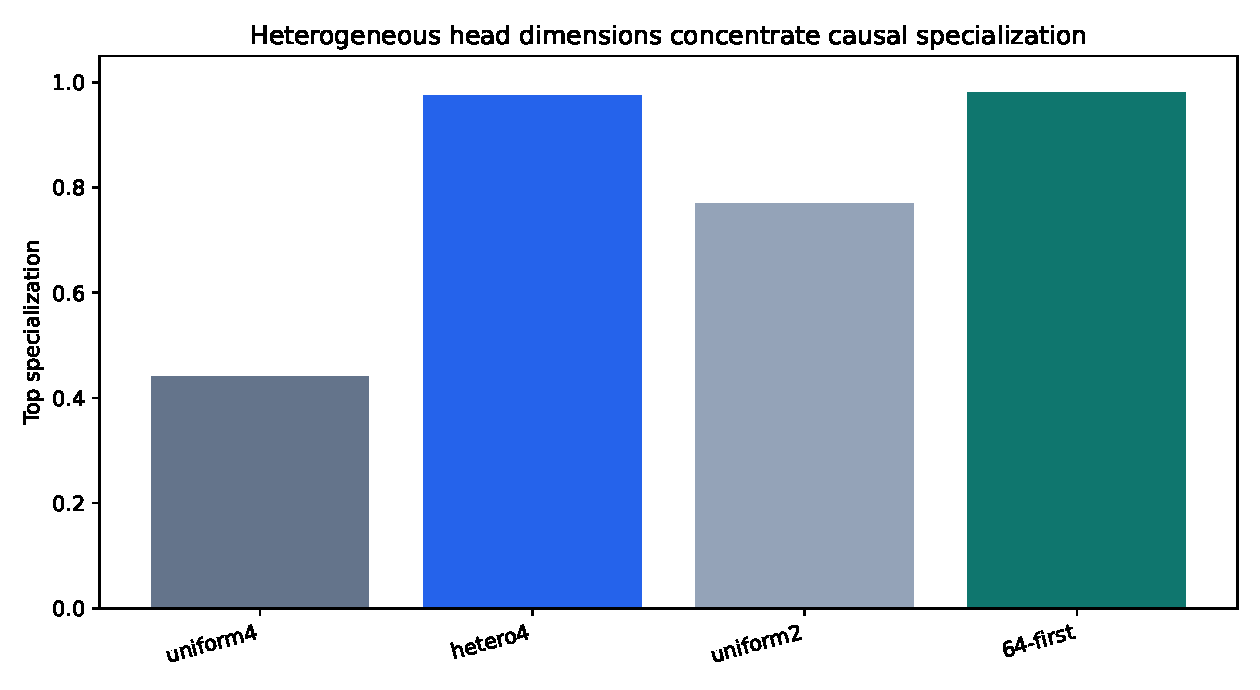
\includegraphics[width=0.88\linewidth]{figures/top_specialization.pdf}
\end{frame}

\begin{frame}{Causal Load}
  \centering
  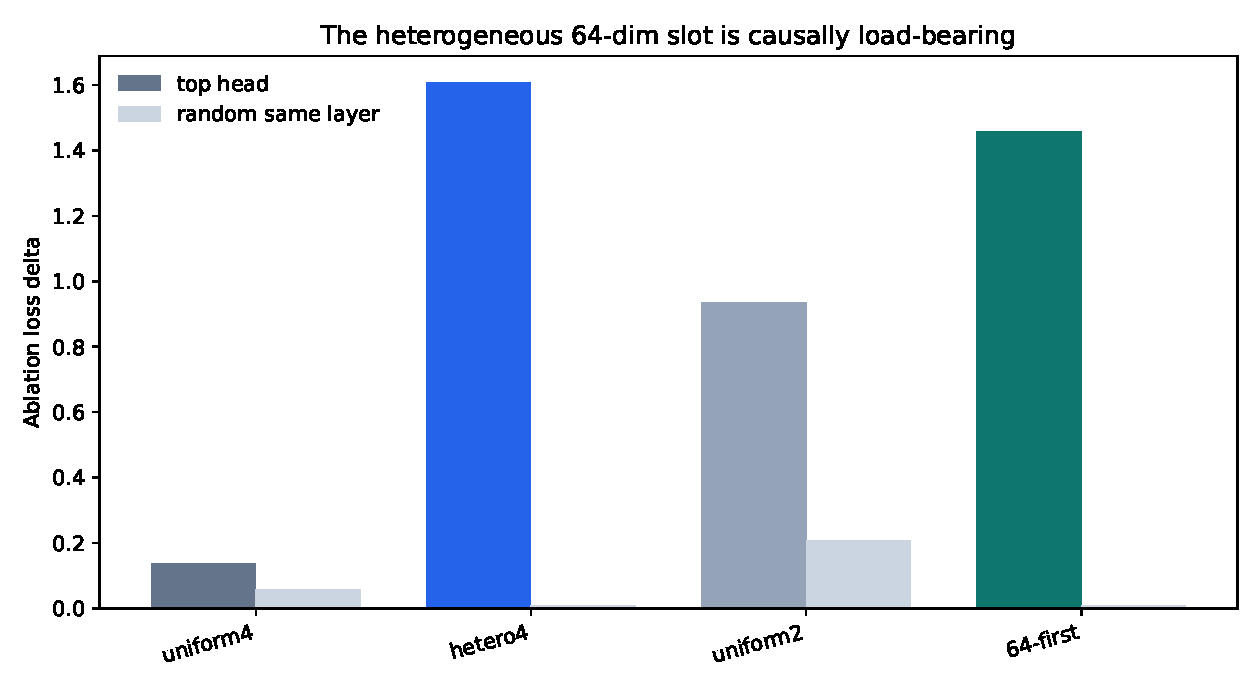
\includegraphics[width=0.88\linewidth]{figures/ablation_delta.pdf}
\end{frame}

\begin{frame}{Cross-Seed Stability}
  \centering
  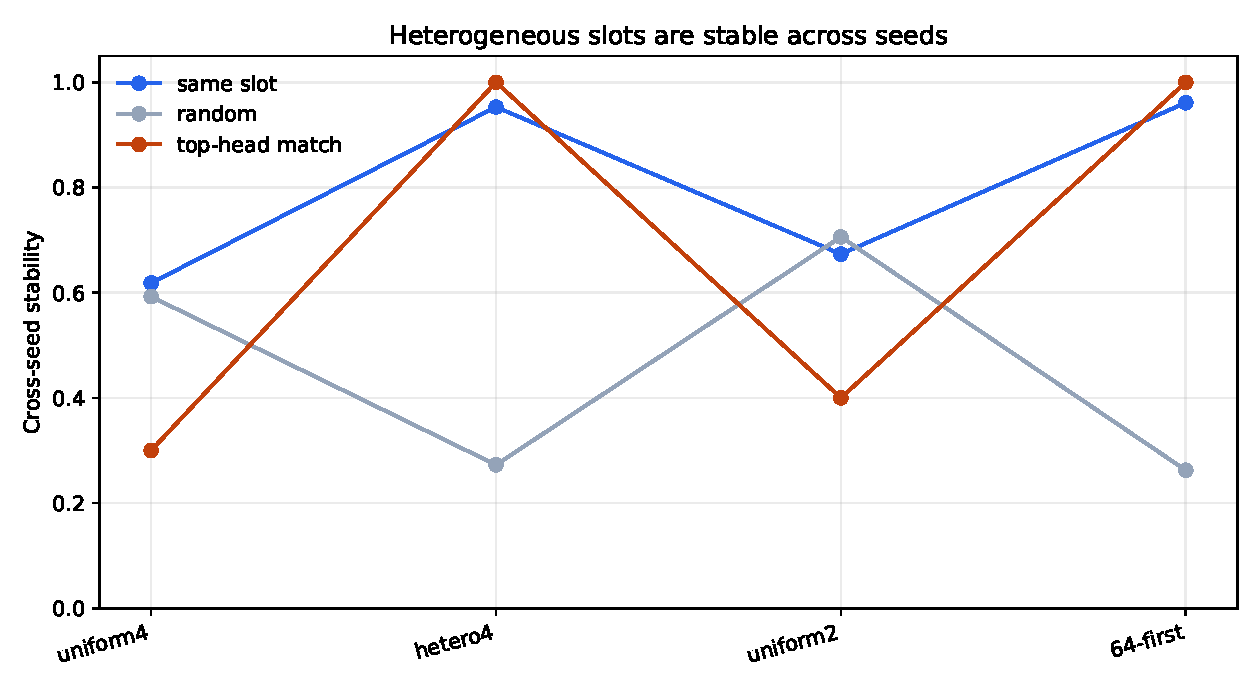
\includegraphics[width=0.88\linewidth]{figures/stability_metrics.pdf}
\end{frame}

\begin{frame}{Position Control}
  \centering
  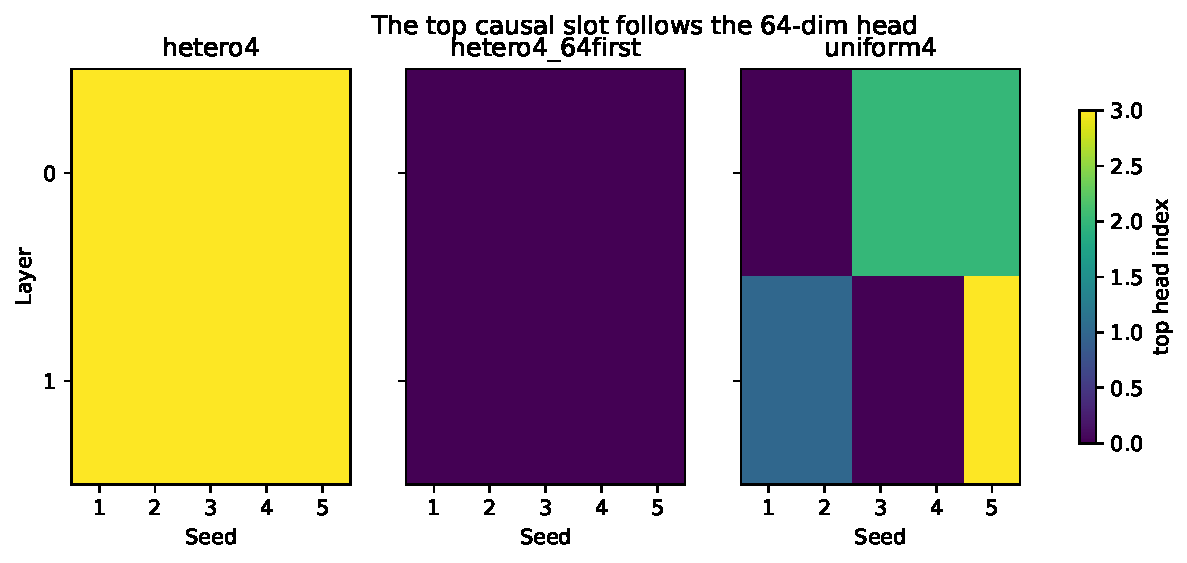
\includegraphics[width=0.88\linewidth]{figures/top_head_slots.pdf}
\end{frame}

\begin{frame}{Interpretation}
  Findings:
  \begin{itemize}
    \item Heterogeneous head dimensions produce a near-single-head causal solution.
    \item The top causal role follows the 64-dim head when its index changes.
    \item Uniform fewer/wider heads help, but do not give the same stable slot.
    \item In heterogeneous architectures, same-slot matching can be more meaningful
      than unconstrained Hungarian matching.
  \end{itemize}
\end{frame}

\begin{frame}{Decision}
  Continue the architectural-intervention branch.

  \vspace{0.8em}
  Next decisive experiment:
  \begin{itemize}
    \item scale this to a richer toy or small LM objective;
    \item keep uniform same-head-count, heterogeneous, and uniform fewer/wider controls;
    \item report same-slot and Hungarian-aligned stability side by side.
  \end{itemize}
\end{frame}

\begin{frame}{Provenance}
  \begin{itemize}
    \item Script: \texttt{scripts/toy\_head\_dim\_intervention.py}
    \item Main output: \texttt{results/phase3\_toy\_head\_dim\_intervention}
    \item Position control: \texttt{results/phase3\_toy\_head\_dim\_position\_control}
    \item Report: \texttt{doc/phase3\_toy\_head\_dim\_intervention.md}
    \item Data copied into this deck folder under \texttt{data/}
  \end{itemize}
\end{frame}

\end{document}
